\begin{figure}
	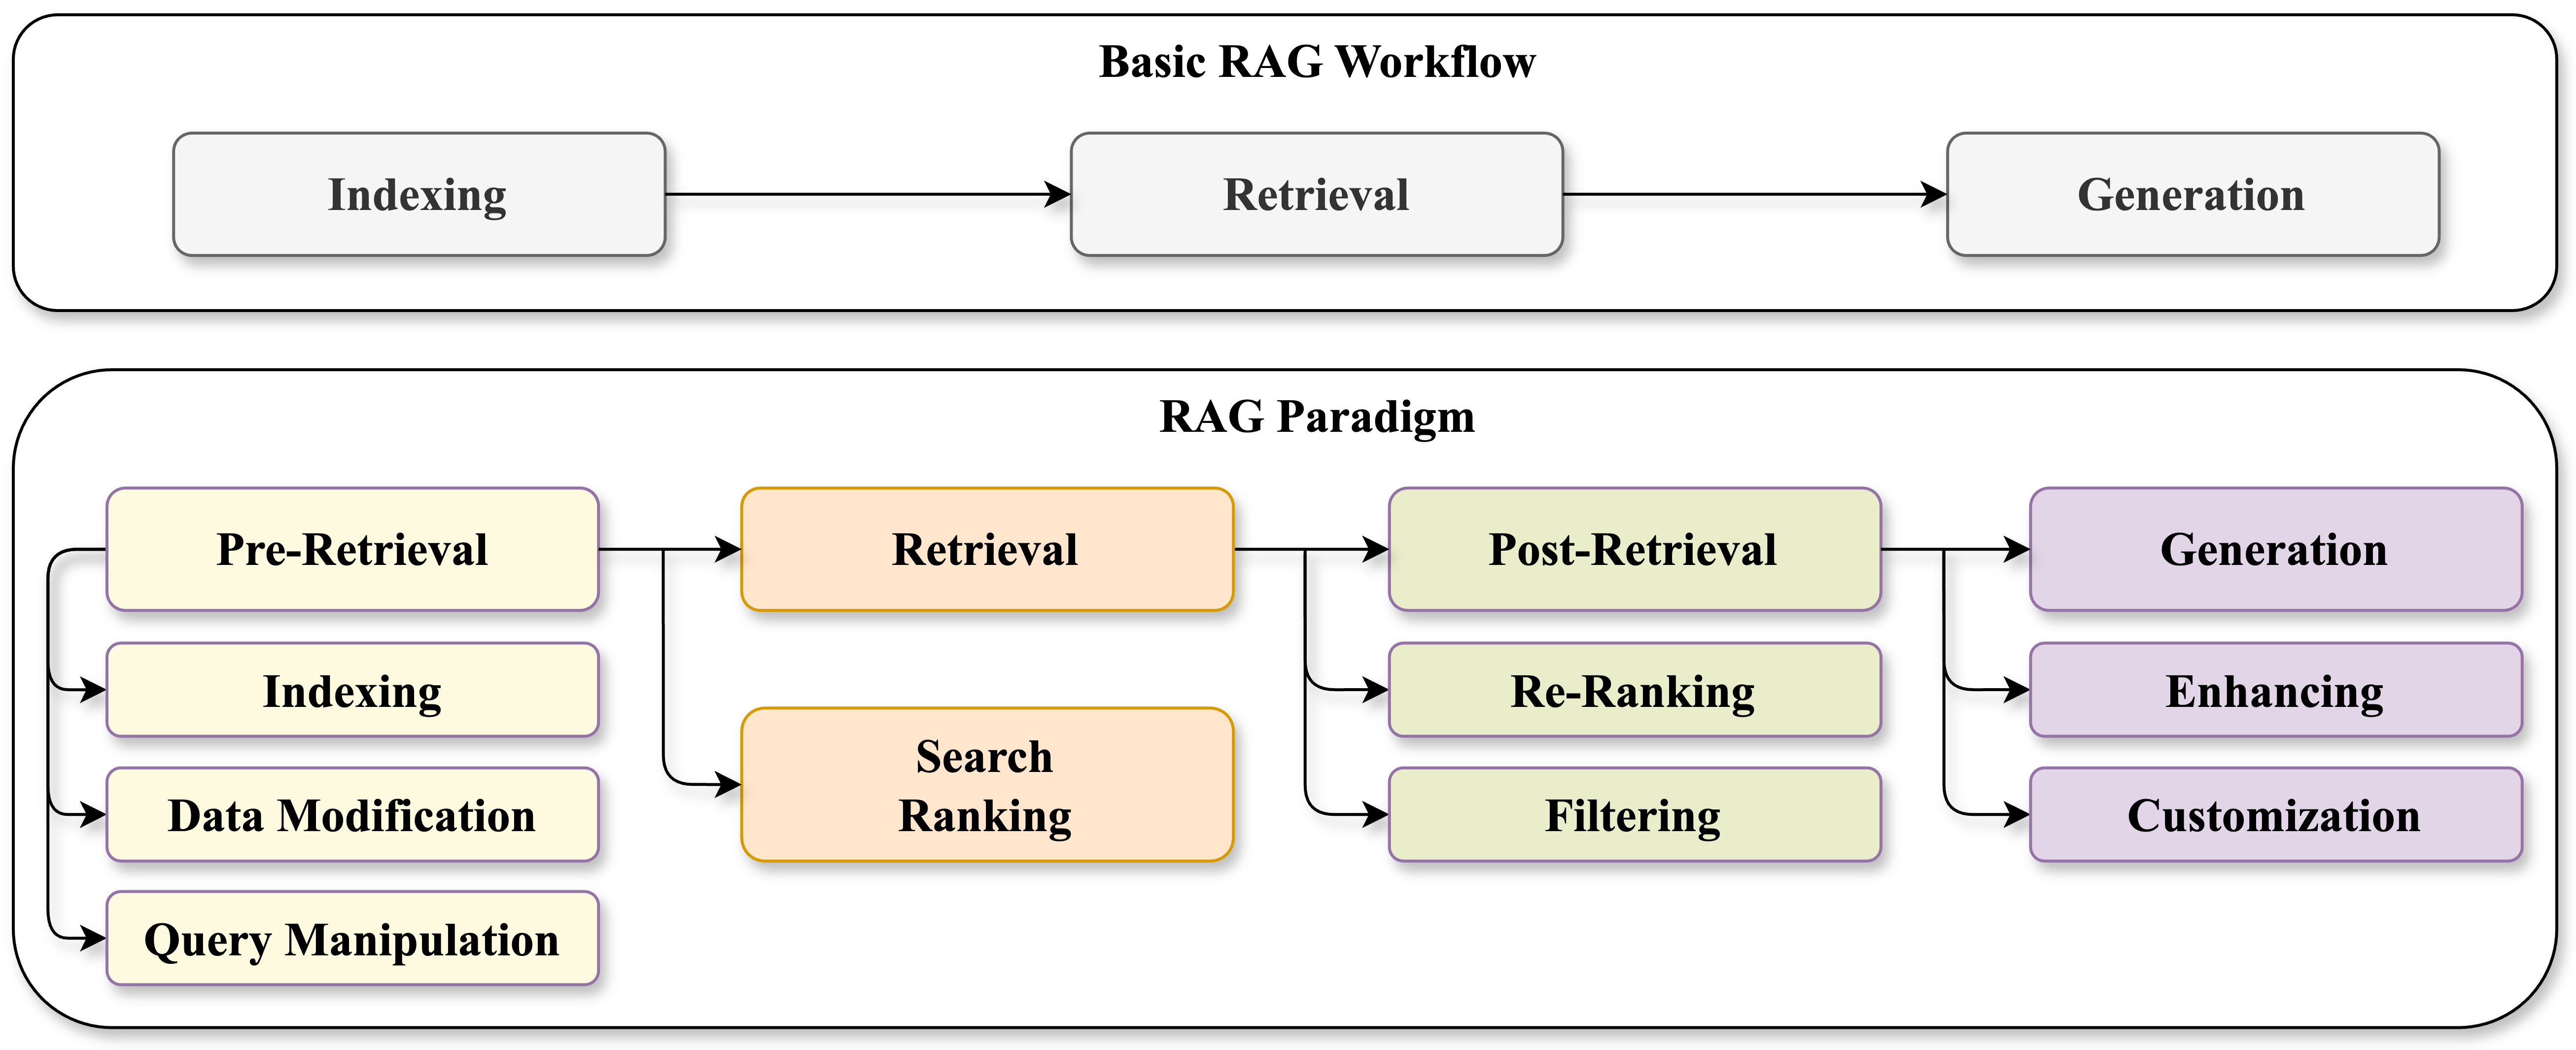
\includegraphics[width=\textwidth]{Figures/RAG_paradigm.png}
	\caption{The unified RAG core concepts with basic workflow.}
	\label{fig:rag_paradigm}
\end{figure}

The hallucinations are largely attributed to LLMs' inability to access up-to-date information. This limitation stems from the models' reliance on their training datasets. RAG proposes a solution to this issue by supplementing the LLM's training data with current information from external sources through a retrieval model, thereby enabling the generation of accurate responses. RAG presents a more cost-effective alternative to the extensive training and fine-tuning processes typically required for LLMs. It allows for the dynamic incorporation of fresh information via traditional retrieval methods or pre-trained LMs, without the need to directly integrate this new data into the LLM. This feature makes RAG both flexible and scalable, facilitating its application across different LLMs for various purposes. The information retrieved through RAG is derived from real-world data, authored by humans, which not only simplifies the generation process but also increases the reliability of the generated responses. 

Research by Khandelwal et al. \cite{khandelwal2020generalization} demonstrates that accessing relevant information from the training dataset itself can significantly improve LLM performance, highlighting the effectiveness of RAG. Over time, RAG has evolved from a means of providing supplementary information to enabling multiple interactions between the retrieval and generation components. This involves conducting several rounds of retrieval to refine the accuracy of the information retrieved and iteratively improve the quality of the generated output. Toolkits such as LangChain\footnote{https://www.langchain.com} and LlamaIndex\footnote{https://www.llamaindex.ai} have modularized the RAG approach, enhancing its adaptability and expanding its range of applications. Despite these toolkits employing diverse methodologies to tackle different aspects of RAG—from multiple search iterations to iterative generation—they maintain adherence to the fundamental RAG workflow. This consistency is crucial for understanding their operation and pinpointing opportunities for further development.

\subsection{Basic RAG Workflow}
 Figure \ref{fig:rag_paradigm} represents the unified RAG core concepts with basic workflow. The workflow of RAG begins with the creation of an index comprising external sources. This index serves as the basis for retrieving relevant information through a retriever model based on a specific query. The final step involves a generator model, which combines the retrieved information with the query to produce the desired output. 

\subsubsection{Indexing}
Efficient retrieval begins with comprehensive indexing, where data preparation is key. This stage involves text normalization processes such as tokenization, stemming, and the removal of stop words to enhance the text's suitability for indexing \cite{DBLP:books/daglib/0021593}. Text segments are then organized into sentences or paragraphs to facilitate more focused searches, allowing for the pinpointing of segments containing pertinent keywords. The integration of deep learning has revolutionized indexing through the use of pretrained LMs for generating semantic vector representations of texts. These vectors are stored, enabling rapid and precise retrieval from extensive data collections, significantly enhancing retrieval efficiency.

\subsubsection{Retrieval}
While traditional retrieval methods, such as the BM25 algorithm \cite{DBLP:conf/trec/Hancock-BeaulieuGHRWW96}, focus on term frequency and presence for document ranking, they often overlook the semantic information of queries. Current strategies leverage pretrained LMs like BERT \cite{devlin2019bert}, which capture the semantic essence of queries more effectively. These models improve search accuracy by considering synonyms and the structure of phrases, thereby refining document ranking through the detection of semantic similarities. This is typically achieved by measuring vector distances between documents and queries, combining traditional retrieval metrics with semantic understanding to yield search results that are both relevant and aligned with user intent.

\subsubsection{Generation}
The generation phase is tasked with producing text that is both relevant to the query and reflective of the information found in the retrieved documents. The usual method involves concatenating the query with the retrieved information, which is then fed into an LLM for text generation \cite{li2022survey}. Although ensuring the generated text's alignment and accuracy with the retrieved content presents challenges, it is also essential to strike a balance between adhering closely to the source material and infusing the output with creativity. The generated text should accurately convey the information from the retrieved documents and align with the query's intent, while also offering the flexibility to introduce new insights or perspectives not explicitly contained within the retrieved data.

\subsection{RAG Paradigm}
The RAG paradigm organizes research within the domain, offering a straightforward yet robust framework to enhance LLM performance. Central to RAG is its search mechanism, crucial for generating high-quality outcomes. Therefore, this paradigm is structured into four main phases from a retrieval perspective: pre-retrieval, retrieval, post-retrieval, and generation. Both single-hop and multi-hop retrieval approaches, encompassing iterative retrieve-generate cycles, follow this four-phase structure. Figure \ref{fig:rag tax} is the taxonomy tree of RAG's core techniques.

\subsubsection{Pre-Retrieval}
The pre-retrieval phase of retrieval-augmented generation lays the foundation for successful data and query preparation, ensuring efficient information retrieval. This phase includes essential tasks to prepare for effective data access.

\paragraph{Indexing} The process starts with indexing, which establishes an organized system to enable fast and accurate retrieval of information. The specificity of indexing depends on the task and data type. For example, sentence-level indexing is beneficial for question-answering systems to precisely locate answers, while document-level indexing is more appropriate for summarizing documents to understand their main concepts and ideas.

\paragraph{Query Manipulation} After indexing, query manipulation is performed to adjust user queries for a better match with the indexed data. This involves query reformulation \cite{DBLP:journals/jasis/JansenBS09, DBLP:conf/sigir/YuLYXBG020}, which rewrites the query to align more closely with the user's intention; query expansion \cite{DBLP:journals/ipm/HuangMH13}, which extends the query to capture more relevant results through synonyms or related terms; and query normalization, which resolves differences in spelling or terminology for consistent query matching.

\paragraph{Data Modification} Data modification is also critical in enhancing retrieval efficiency. This step includes preprocessing techniques like removing irrelevant or redundant information to improve the quality of results and enriching the data with additional information such as metadata to boost the relevance and diversity of the retrieved content \cite{DBLP:conf/nips/BevilacquaOLY0P22}.

\subsubsection{Retrieval}
\paragraph{Search \& Ranking} The retrieval stage is the combination of search and ranking. It focuses on selecting and prioritizing documents from a dataset to enhance the quality of the generation model's outputs. This stage employs search algorithms to navigate through the indexed data, finding documents that match a user's query.  After identifying relevant documents, the process of initially ranking these documents starts to sort them according to their relevance to the query. 

\subsubsection{Post-Retrieval}
The post-retrieval phase serves to refine the initially retrieved documents to improve the quality of text generation. This phase consists of re-ranking and filtering, each aimed at optimizing the document selection for the final generation task.

\paragraph{Re-Ranking}
In the re-ranking step, the documents previously retrieved are reassessed, scored, and reorganized. The objective is to more accurately highlight the documents most relevant to the query and diminish the importance of the less relevant ones. This step involves incorporating additional metrics and external knowledge sources to enhance precision. In this context, pre-trained models with superior accuracy but lower efficiency can be effectively employed due to the limited set of candidate documents available \cite{DBLP:conf/sigir/HuangH09}. 

\paragraph{Filtering} Filtering aims to remove documents that fail to meet specified quality or relevance standards \cite{khattab2020colbert, DBLP:conf/ecai/HuangH23}. This can be done through several approaches, such as establishing a minimum relevance score threshold to exclude documents below a certain relevance level. Furthermore, the use of feedback from users or prior relevance evaluations assists in adjusting the filtering process, guaranteeing that only the most relevant documents are retained for text generation.

\subsubsection{Generation}
The generation stage is a crucial component of the RAG process, responsible for leveraging retrieved information to enhance the quality of the generated response. This stage encompasses several sub-steps aimed at producing content that is readable, engaging, and informative.

\paragraph{Enhancing}
At the heart of the generation phase is the enhancement step, where the objective is to merge the retrieved information with the user's query to create a coherent and relevant response. This includes the process of elaboration, adding extra details to the retrieved content to enrich it. Efforts are focused on improving the output's quality by increasing its clarity, coherence, and stylistic appeal through methods such as rephrasing and restructuring. Information from various sources is combined to offer a comprehensive perspective, and verification is conducted to ensure the accuracy and relevance of the content.

\paragraph{Customization}
Customization is user-centric. It encompasses tailoring content in two primary ways. First, it aligns the generated output with relevant information retrieved in earlier stages, ensuring consistency and accuracy by incorporating key knowledge. Second, it adapts the content to suit user-specific factors such as intended audience, situational context, and personal preferences, shaping the response to be both contextually relevant and user-centric. This dual focus on integrating relevant knowledge and adjusting to diverse contextual demands forms the basis of effective customization in RAG.